\documentclass[aspectratio=169,10pt]{beamer}

% ----------------------------------------------------------------------
% Design System Review Presentation — Nexa Design Guild
% ----------------------------------------------------------------------
\usepackage[utf8]{inputenc}
\usepackage[T1]{fontenc}
\usepackage{lmodern}
\usepackage{xcolor}
\usepackage{booktabs}
\usepackage{array}
\usepackage{tikz}
\usetikzlibrary{positioning,calc,shapes.geometric,arrows.meta,backgrounds}
\usepackage{pgfplots}
\pgfplotsset{compat=1.17}
\usepackage{tcolorbox}
\tcbuselibrary{skins}
\usepackage{hyperref}

% ----------------------------------------------------------------------
% Palette
% ----------------------------------------------------------------------
\definecolor{nexaink}{RGB}{20,24,31}
\definecolor{nexateal}{RGB}{0,121,107}
\definecolor{nexaamber}{RGB}{230,159,0}
\definecolor{nexagray}{RGB}{110,118,129}
\definecolor{nexacanvas}{RGB}{250,250,248}

% ----------------------------------------------------------------------
% Beamer theme wiring
% ----------------------------------------------------------------------
\usetheme{default}
\usefonttheme{professionalfonts}
\setbeamertemplate{navigation symbols}{}
\setbeamercolor{normal text}{fg=nexaink,bg=nexacanvas}
\setbeamercolor{background canvas}{bg=nexacanvas}
\setbeamercolor{frametitle}{fg=nexacanvas,bg=nexateal}
\setbeamercolor{title}{fg=nexateal}
\setbeamercolor{subtitle}{fg=nexagray}
\setbeamercolor{author}{fg=nexaink}
\setbeamercolor{institute}{fg=nexagray}
\setbeamercolor{section in toc}{fg=nexaink}
\setbeamercolor{itemize item}{fg=nexateal}
\setbeamercolor{itemize subitem}{fg=nexaamber}
\setbeamercolor{block title}{fg=nexacanvas,bg=nexateal}
\setbeamercolor{block body}{fg=nexaink,bg=nexateal!8}
\setbeamerfont{frametitle}{series=\bfseries,size=\Large}
\setbeamertemplate{itemize items}[circle]
\setbeamertemplate{blocks}[rounded][shadow=false]

\setbeamertemplate{footline}{%
  \leavevmode
  \hbox{%
    \begin{beamercolorbox}[wd=.7\paperwidth,ht=2.6ex,dp=1ex,left,leftskip=1em]{author in head/foot}
      {\tiny\color{nexagray}Nexa Design Guild --- Component Library v3.0 Review}
    \end{beamercolorbox}%
    \begin{beamercolorbox}[wd=.3\paperwidth,ht=2.6ex,dp=1ex,right,rightskip=1em]{page number in head/foot}
      {\tiny\color{nexagray}\insertframenumber\,/\,\inserttotalframenumber}
    \end{beamercolorbox}%
  }%
}

\newcommand{\tokenchip}[2]{%
  \tikz[baseline=-0.5ex]\fill[#1] (0,0) rectangle (0.32,0.32);\;#2%
}

\title[Design System Review]{Design System Review}
\subtitle{Nexa Component Library v3.0 --- Token Architecture, Adoption, and Roadmap}
\author{Priya Kapoor \\ \small Staff Design Engineer, Core Platform Pod}
\institute{Nexa Design Guild --- Quarterly Review}
\date{August 2026}

\begin{document}

% ----------------------------------------------------------------------
\begin{frame}
  \titlepage
\end{frame}

% ----------------------------------------------------------------------
\begin{frame}{Agenda}
  \begin{itemize}
    \item Foundations: colour and typography tokens
    \item Token architecture --- how a raw value becomes a component style
    \item Component inventory and stability status
    \item Adoption across product pods
    \item Accessibility posture and open risks
    \item Roadmap and asks for this room
  \end{itemize}
  \vfill
  \begin{block}{Why this review}
    Six months since the v3.0 token rewrite shipped. Time to check whether
    the system is actually being adopted, not just published.
  \end{block}
\end{frame}

% ----------------------------------------------------------------------
\begin{frame}{Foundations --- Colour Tokens}
  \small
  \begin{table}
    \centering
    \renewcommand{\arraystretch}{1.25}
    \begin{tabular}{@{}lllc@{}}
      \toprule
      \textbf{Token} & \textbf{Value} & \textbf{Role} & \textbf{Contrast (on \#FAFAF8)} \\
      \midrule
      \texttt{color.brand.teal.600} & \tokenchip{nexateal}{\#00796B} & Primary action, brand & 4.6:1 \\
      \texttt{color.accent.amber.500} & \tokenchip{nexaamber}{\#E69F00} & Emphasis, warning & 2.9:1$^{\ast}$ \\
      \texttt{color.ink.900} & \tokenchip{nexaink}{\#14181F} & Body text & 15.8:1 \\
      \texttt{color.neutral.500} & \tokenchip{nexagray}{\#6E7681} & Secondary text, borders & 4.9:1 \\
      \texttt{color.surface.canvas} & \tokenchip{nexacanvas}{\#FAFAF8} & Page background & --- \\
      \bottomrule
    \end{tabular}
  \end{table}
  {\scriptsize $^{\ast}$Amber passes WCAG AA only at 18pt+ or 14pt bold; flagged in the
  accessibility section.}
\end{frame}

% ----------------------------------------------------------------------
\begin{frame}{Foundations --- Type Scale}
  \small
  \begin{table}
    \centering
    \renewcommand{\arraystretch}{1.3}
    \begin{tabular}{@{}lccl@{}}
      \toprule
      \textbf{Token} & \textbf{Size / Line} & \textbf{Weight} & \textbf{Usage} \\
      \midrule
      \texttt{type.display} & 40 / 48 & 700 & Hero headings, marketing surfaces \\
      \texttt{type.heading-1} & 28 / 36 & 700 & Page titles \\
      \texttt{type.heading-2} & 22 / 30 & 600 & Section headers, card titles \\
      \texttt{type.body} & 16 / 24 & 400 & Paragraph text, form labels \\
      \texttt{type.caption} & 13 / 18 & 500 & Metadata, timestamps, table cells \\
      \bottomrule
    \end{tabular}
  \end{table}
  \vspace{0.4cm}
  \begin{columns}[T]
    \begin{column}{0.48\textwidth}
      {\large\bfseries\color{nexateal} Aa Design Systems}\\[2pt]
      {\normalsize Every component references a semantic token, never a raw pixel value.}
    \end{column}
    \begin{column}{0.48\textwidth}
      {\scriptsize\color{nexagray}\texttt{type.caption} --- updated 14:02, migrated 3/6 pods}
    \end{column}
  \end{columns}
\end{frame}

% ----------------------------------------------------------------------
\begin{frame}{Token Architecture --- Three Tiers}
  \centering
  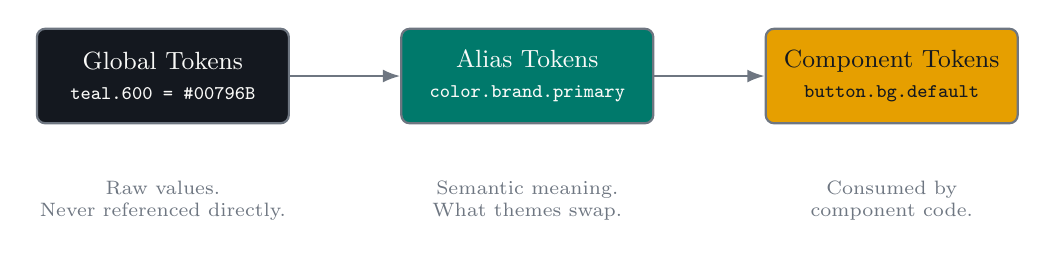
\begin{tikzpicture}[
      node distance=10mm and 14mm,
      tier/.style={rectangle, rounded corners=3pt, minimum width=32mm, minimum height=12mm,
        align=center, draw=nexagray, thick, font=\small},
      arrow/.style={-{Latex[length=2.2mm]}, thick, color=nexagray}
    ]
    \node[tier, fill=nexaink, text=nexacanvas] (global) {Global Tokens\\\texttt{\scriptsize teal.600 = \#00796B}};
    \node[tier, fill=nexateal, text=nexacanvas, right=of global] (alias) {Alias Tokens\\\texttt{\scriptsize color.brand.primary}};
    \node[tier, fill=nexaamber, text=nexaink, right=of alias] (component) {Component Tokens\\\texttt{\scriptsize button.bg.default}};

    \draw[arrow] (global) -- (alias);
    \draw[arrow] (alias) -- (component);

    \node[below=6mm of global, font=\scriptsize, text width=32mm, align=center, color=nexagray]
      {Raw values.\\Never referenced directly.};
    \node[below=6mm of alias, font=\scriptsize, text width=32mm, align=center, color=nexagray]
      {Semantic meaning.\\What themes swap.};
    \node[below=6mm of component, font=\scriptsize, text width=32mm, align=center, color=nexagray]
      {Consumed by\\component code.};
  \end{tikzpicture}
  \vspace{0.5cm}
  \begin{block}{Rule of the system}
    A component may only read from the component tier. If a component reaches past
    it to an alias or global token directly, that is a lint failure, not a style choice.
  \end{block}
\end{frame}

% ----------------------------------------------------------------------
\begin{frame}{Component Inventory}
  \small
  \begin{table}
    \centering
    \renewcommand{\arraystretch}{1.25}
    \begin{tabular}{@{}llll@{}}
      \toprule
      \textbf{Component} & \textbf{Status} & \textbf{Owner Pod} & \textbf{WCAG AA} \\
      \midrule
      Button & Stable v3 & Core Platform & \color{nexateal}Pass \\
      Data Table & Stable v3 & Core Platform & \color{nexateal}Pass \\
      Toast Notification & Stable v2 & Core Platform & \color{nexateal}Pass \\
      Date Picker & Beta v0.9 & Synapse Pod & \color{nexaamber}Partial \\
      Command Palette & Beta v0.4 & Vertex Pod & \color{nexateal}Pass \\
      Rich Text Editor & Deprecated & Nimbus Pod & Fail (removal Q4) \\
      \bottomrule
    \end{tabular}
  \end{table}
  \vfill
  {\scriptsize\color{nexagray}Status legend: \textbf{Stable} --- API frozen, semver guaranteed.
  \textbf{Beta} --- API may change with a deprecation window.
  \textbf{Deprecated} --- scheduled for removal, do not adopt in new work.}
\end{frame}

% ----------------------------------------------------------------------
\begin{frame}{Adoption Across Pods}
  \centering
  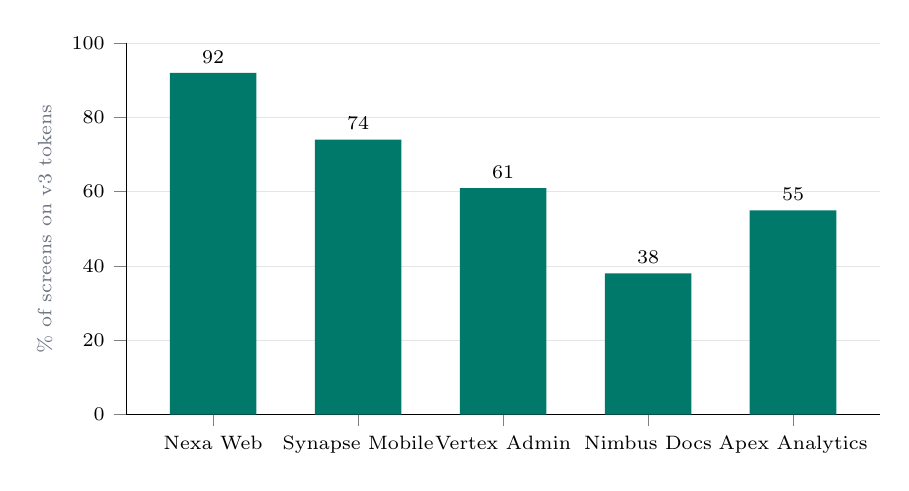
\begin{tikzpicture}
    \begin{axis}[
        width=0.92\textwidth, height=6.3cm,
        ybar, bar width=11mm,
        ymin=0, ymax=100,
        ylabel={\% of screens on v3 tokens},
        ylabel style={font=\scriptsize, color=nexagray},
        symbolic x coords={Nexa Web,Synapse Mobile,Vertex Admin,Nimbus Docs,Apex Analytics},
        xtick=data,
        x tick label style={font=\scriptsize},
        y tick label style={font=\scriptsize},
        nodes near coords, nodes near coords style={font=\scriptsize},
        axis lines*=left,
        enlarge x limits=0.15,
        ymajorgrids, grid style={gray!20},
        tick align=outside,
      ]
      \addplot[fill=nexateal, draw=none] coordinates {
        (Nexa Web,92) (Synapse Mobile,74) (Vertex Admin,61) (Nimbus Docs,38) (Apex Analytics,55)
      };
    \end{axis}
  \end{tikzpicture}
  \vspace{0.2cm}
  {\scriptsize\color{nexagray}Nimbus Docs is the outlier --- still on a forked v2 button
  component pending the Rich Text Editor deprecation.}
\end{frame}

% ----------------------------------------------------------------------
\begin{frame}{Accessibility Posture}
  \begin{columns}[T]
    \begin{column}{0.48\textwidth}
      \begin{tcolorbox}[colback=nexateal!8, colframe=nexateal, title=Holding the line,
          fonttitle=\bfseries\small, coltitle=nexacanvas, boxrule=0.6pt, arc=2pt]
        \small
        \begin{itemize}
          \item All Core Platform components pass WCAG 2.1 AA contrast checks
          \item Focus rings ship as a component token, not an override
          \item Keyboard nav covered by the shared test harness
        \end{itemize}
      \end{tcolorbox}
    \end{column}
    \begin{column}{0.48\textwidth}
      \begin{tcolorbox}[colback=nexaamber!12, colframe=nexaamber, title=Open risks,
          fonttitle=\bfseries\small, coltitle=nexaink, boxrule=0.6pt, arc=2pt]
        \small
        \begin{itemize}
          \item Amber accent fails AA below 18pt --- used in three Synapse alerts
          \item Date Picker beta lacks a screen-reader label for range mode
          \item Rich Text Editor has no accessible toolbar; do not extend usage
        \end{itemize}
      \end{tcolorbox}
    \end{column}
  \end{columns}
  \vfill
  \par
  {\scriptsize\color{nexagray}Full audit trail: \texttt{design-guild/a11y-log}, reviewed monthly
  by the Core Platform pod.}
\end{frame}

% ----------------------------------------------------------------------
\begin{frame}{Roadmap --- Next Two Quarters}
  \small
  \begin{itemize}
    \item[\textbf{Q3 2026}] Ship Date Picker v1.0; close the amber contrast gap with a
      \texttt{color.accent.amber.700} token for small text
    \item[\textbf{Q3 2026}] Migrate Nimbus Docs off the forked button; retire the fork
      in the shared repo
    \item[\textbf{Q4 2026}] Remove Rich Text Editor; replace with the Meridian-contributed
      block editor currently in incubation
    \item[\textbf{Q4 2026}] Command Palette to Stable, pending Vertex Pod's keyboard
      shortcut audit
    \item[\textbf{Q1 2027}] Publish token architecture as an open package for teams
      outside the guild to consume directly
  \end{itemize}
\end{frame}

% ----------------------------------------------------------------------
\begin{frame}{Discussion}
  \centering
  \vspace{0.6cm}
  {\Large\bfseries\color{nexateal} Questions, pushback, adoption blockers}
  \vspace{0.8cm}

  \begin{tabular}{@{}ll@{}}
    \textbf{Priya Kapoor} & Staff Design Engineer, Core Platform Pod \\
    \textbf{Design Guild channel} & \texttt{\#nexa-design-guild} \\
    \textbf{Token repo} & \texttt{github.com/nexa/design-tokens} \\
  \end{tabular}

  \vspace{1cm}
  {\scriptsize\color{nexagray}Slides and the full audit trail are posted to the guild wiki
  after this session.}
\end{frame}

\end{document}
